\documentclass[a4paper, 12pt]{article} % тип документа

%%%Библиотеки
	%\usepackage[warn]{mathtext}	
	%\usepackage[T2A]{fontenc}   %Кодировка
	\usepackage[utf8]{inputenc} %Кодировка исходного текста
	\usepackage[english, russian]{babel} %Локализация и переносы
	\usepackage{caption}
	\usepackage{listings}
	\usepackage{amsmath, amsfonts, amssymb, amsthm, mathtools}
	\usepackage[warn]{mathtext}
	\usepackage[mathscr]{eucal}
	\usepackage{wasysym}
	\usepackage{graphicx} %Вставка картинок правильная
	\usepackage{indentfirst}
	\usepackage{float}    %Плавающие картинки
	\usepackage{wrapfig}  %Обтекание фигур (таблиц, картинок и прочего)
	\usepackage{fancyhdr} %Загрузим пакет
	\usepackage{lscape}
	\usepackage{xcolor}
	\usepackage[normalem]{ulem}
	
	\usepackage{titlesec}
	\titlelabel{\thetitle.\quad}

	\usepackage{hyperref}

%%%Конец библиотек

%%%Настройка ссылок
	\hypersetup
	{
		colorlinks = true,
		linkcolor  = blue,
		filecolor  = magenta,
		urlcolor   = blue
	}
%%%Конец настройки ссылок


%%%Настройка колонтитулы
	\pagestyle{fancy}
	\fancyhead{}
	\fancyhead[L]{2.3.1}
	\fancyhead[R]{Талашкевич Даниил, группа Б01-009}
	\fancyfoot[C]{\thepage}
%%%конец настройки колонтитулы



\begin{document}
						%%%%Начало документа%%%%


%%%Начало титульника
\begin{titlepage}

	\newpage
	\begin{center}
		\normalsize Московский физико-технический институт \\(госудраственный университет)
	\end{center}

	\vspace{6em}

	\begin{center}
		\Large Лабораторная работа по общему курсу физики\\Термодинамика и молекулярная физика
	\end{center}

	\vspace{1em}

	\begin{center}
		\Large \textbf{2.3.1. Современные средства
получения и измерения вакуума}
	\end{center}

	\vspace{2em}

	\begin{center}
		\large Талашкевич Даниил Александрович\\
		Группа Б01-009
	\end{center}

	\vspace{\fill}

	\begin{center}
		Долгопрудный \\2021
	\end{center}
	
\end{titlepage}
%%%Конец Титульника



%%%Настройка оглавления и нумерации страниц
	\thispagestyle{empty}
	\newpage
	\tableofcontents
	\newpage
	\setcounter{page}{1}
%%%Настройка оглавления и нумерации страниц


					%%%%%%Начало работы с текстом%%%%%%

\textbf{Цель работы:} 1) измерение объемов форвакуумной и высоковакуумной частей установки; 2) определение скорости откачки системы в стационарном режиме, а также по ухудшению и улучшению вакуума.\\

\textbf{Используемое оборудование:} вакуумная установка с манометрами: масляным, термопарным и ионизационным.

\section{Теоретические сведения}
\subsection{Введение}

В физике вакуумом называют состояние газа, при котором характерная длина свободного пробега молекул в газе $\lambda$ сравнима по порядку
величины с характерным линейным размером сосуда $d$, в котором газ
находится.

Основы процесса откачки и связанные с ним понятия рассмотрим
на примере простейшей вакуумной системы.

Предельное остаточное давление (предельный вакуум) $P_{\text{пр}}$ -- наименьшее давление газа, которое формируется в процессе откачки в рассматриваемом сечении вакуумпровода (рассматриваемой точке вакуумной системы). Обычно выделяют предельное давление в
камере или на входе в насос.

Наибольшее выпускное давление -- максимально допустимое давление газа на входе насоса.

\begin{figure}[h]
    \centering
    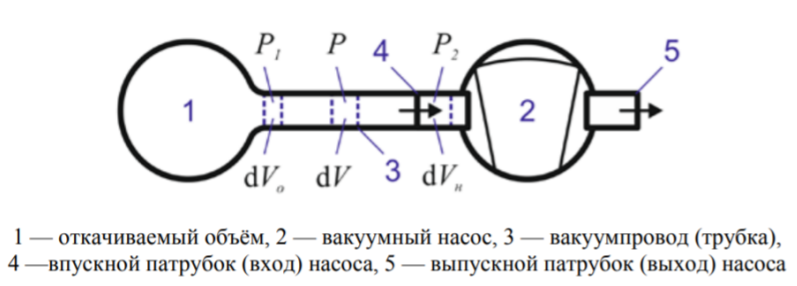
\includegraphics[width = 11 cm]{1png.png}
    \caption{Простейшая вакуумная система}
    \label{fig:vac}
\end{figure}

Быстрота откачивающего действия (скорость откачки) вакуумной системы $S$ -- объем газа, проходящий через рассматриваемое сечение вакуумпровода в единицу времени при текущем давлении
в данном сечении:
 
\begin{equation}
	S = \frac{dV}{dT}
\end{equation}

Следовательно, быстродействие насоса $S_{\text{н}}$ определяется как:

\begin{equation}
	S_{\text{н}} = \frac{dV_{\text{н}}}{dT}
\end{equation}

а эффективная скорость откачки камеры $S_{\text{o}}$:

\begin{equation}
	S_{\text{o}} = \frac{dV_{\text{o}}}{dT}
\end{equation}

Падение давления вдоль вакуумпровода $\Delta P = P_1 - P_2$ определяется его пропускной способностью (проводимостью) $U$:

\begin{equation}
	U = \frac{Q}{P_1 - P_2}
\end{equation}
где $Q$ -- поток газа через вакуумпровод с соответствующими
давлениями на концах.

Величина $Z$, обратная проводимости, называется импедансом вакуумпровода:

\begin{equation}
	Z = \frac{1}{U}
\end{equation}

В общем случае указанные величины $S, U, Q, Z$ как и сами давления $P_1$ и $P_2$ зависят от времени. Но в конце процесса откачки устанавливается квазистационарный режим, при котором поток газа становится практически постоянным и равным количеству поступающего в систему газа
в единицу времени вследствие наличия течей, т.е. нарушения герметичности (в основном в местах механического соединения отдельных узлов
вакуумной системы). Для стационарного режима можно записать условие
непрерывности потока откачиваемого газа:

\begin{equation}
	P_1S_{\text{o}} = PS = P_2S_{\text{н}} = Q
\end{equation}

Из предыдущих уравнений легко получить, что

\begin{equation}
	\frac{1}{S_{\text{o}}} = \frac{1}{S_{\text{н}}} + \frac{1}{U}
\end{equation}

Это уравнение позволяет правильно ориентироваться в выборе средств
откачки и вакуумпроводов при конструировании вакуумной системы для
любых целей.

Количественной характеристикой течи, является натекание $Q_{\text{н}}$, измеряемое при отключенных средствах откачки:

\begin{equation}
	Q_{\text{н}} = V \frac{P_{\text{к}} - P_{\text{н}}}{\Delta t}
\end{equation}
где $V$ -- замкнутый исследуемый объём; $P_{\text{н}}$, $P_{\text{к}}$ -- начальное и конечное давление в объеме; $\Delta t$ -- время между измерениями давления. При наличии течей, нормальной работе средств откачки и отсутствии в системе
источников паров или газов, зависимость потока газа через течь от времени $Q_{\text{н}}(t)$ носит, как правило, линейный характер.

Для заданного давления $P_1$ в замкнутом исследуемом объёме допустимым считается натекание:

\begin{equation}
	Q_{\text{н}} \ll Q = P_1 S_{\text{o}} = P_1 \frac{S_{\text{н}} U}{S_{\text{н}} + U}
\end{equation}

На пропускную способность вакуумпровода существенно влияет
режим течения газа, который характеризуется числом Кнудсена, равным
отношению длины свободного пробега молекул в газе к характерному
линейному размеру течения:

\begin{equation}
	Kn = \frac{\lambda}{d}
\end{equation}

Данная величина характеризует степень разреженности газового
потока:
\begin{enumerate}

	\item В гидродинамическом (вязкостном) режиме течения ($Kn \ll 1$)
различают ламинарные и турбулентные потоки. При ламинарном
течении молекулы газа движутся по параллельным траекториям
со скоростями, мало отличающимися друг от друга. При турбулентном течении наряду с поступательным движением всей массы газа, молекулы движутся хаотически со скоростями, подвергающимися случайным изменениям

	\item В молекулярном (кнудсеновском) режиме ($Kn \gg 1$) течение газа
сводится к независимому движению отдельных молекул по прямым линиям в периоды между соударениями главным образом со
стенками вакуумпровода.

	\item В переходном режиме ($Kn \thicksim 1$) в системе могут существовать все
описанные выше виды течения.

\end{enumerate}

В разных режимах течения пропускная способность вакуумпровода имеет существенно различные зависимости от размера его поперечного сечения.

\subsection{Проводимость отверстия в стенке}

В кнудсеновском режиме проводимость отверстия радиусом $R$
определяется средним числом молекул, сталкивающихся со стенкой. С точки зрения молекулярно-кинетической теории можно получить

\begin{equation}
	\nu = \nu_2 - \nu_1 = \frac{v}{4kT} (P_2 - P_1)
\end{equation}

С другой стороны 

\begin{equation}
	\nu = \frac{1}{AkT} (P_2 - P_1) U_{\text{отв}}
\end{equation}

Из формул слеудет, что

\begin{equation}
	U_{\text{{отв}}} = \frac{Av}{4} = \frac{\pi R^2}{4} \sqrt{\frac{8kT}{\pi m}}
\end{equation}


\subsection{Проводимость длинного трубопровода}

Проводимость длинного трубопровода $L \gg R$ в гидродинамическом режиме определяется вязкостными характеристиками газа и может
быть получена из формулы Пуазейля

\begin{equation}
	U_{\text{тр}} = \frac{Q}{P_2 - P_1} = P  \frac{\pi R^4}{8 \mu L} \thicksim \frac{R^4}{L} \frac{P}{\sqrt{Tm}}
\end{equation}

где $P$ -- давление в рассматриваемом сечении трубы (можно рассматривать как среднее по длине вакуумпровода давление $P = (P_1 + P_2)/2$, $\mu$ -- вязкость газа, $L$ и $R$ -- длина и радиусс трубопровода.

В молекулярном режиме проводимость определяется взаимодействием молекул газа со стенками и может быть получена из формулы
Кнудсена

\begin{equation}
	U_{\text{тр}} = \frac{Q}{P_2 - P_1} = \frac{4}{3} \frac{R^3}{L} \sqrt{\frac{2 \pi k T}{m}} \thicksim \frac{R^3}{L} \sqrt{\frac{T}{m}}
\end{equation}

Для промежуточных условий проводимость определяется путём
интерполяции зависимостей, полученных в вязкостном и молекулярном
режимах.

В случае последовательного соединения разных вакуумпроводов,
что обычно бывает в реальных установках, их импедансы суммируются,
а суммарная проводимость равна:

\begin{equation}
	U_{\Sigma} = \frac{1}{\Sigma Z_{i}}
\end{equation}

Формулы показывают, что для эффективной
откачки вакуумной камеры насосом с заданной скоростью откачки нужно
выбирать вакуумпроводы как можно шире и как можно короче. В этом
случае $U_{\Sigma} \gg S_{\text{н}}$:

\begin{equation}
	S_{\text{o}} = \frac{S_{\text{н}} U}{S_{\text{н}} + U} = S_{\text{н}}
\end{equation}

\subsection{Время откачки}

Положим, что за промежуток времени $dt$ давление
в откачиваемом объёме $V_{\text{o}}$ снижается на $dP_1$. Тогда за промежуток времени $dt$ количество газа поступающего в трубку равно $S_{\text{o}} P_1 dt$, а эта же
убыль газа в объеме равна $V_{\text{o}} dP_1$, следовательно:

\begin{equation}
	dt = - \frac{V_{\text{o}} dP_1}{S_{\text{o}}P_1}
\end{equation}

В случае $S_{\text{o}} = const$ иммем 

\begin{equation}
	P(t) = P_1 \exp \left( - \frac{S_{\text{o}}}{V_{\text{o}}}t \right)
\end{equation}


\section{Экспериментальная установка и методика работы}

Существует множество различных типов вакуумных насосов, целесообразность использования которых варьируется в зависимости от условий получения и требуемой глубины вакуума.

\subsection{Мембранный (диафрагменный) насос}

В мембранном насосе две или более гибких диафрагмы жестко закреплены на стенках корпуса, образуя герметичные полости изменяемого объема. Диафрагмы приводятся в движение
электродвигателем, вращательное движение которого преобразуется
в возвратно-поступательное с использованием кривошипно-шатунного
механизма. С движением диафрагмы синхронизирована работа
впускного и выпускного клапанов. Откачка осуществляется созданием
в полости диафрагмы области пониженного давления, за счет чего в нее через впускной клапан поступает газ из откачиваемого объема или предыдущей ступени откачки. При уменьшении объема полости газ уходит через выпускной клапан.

\begin{figure}[h]
    \centering
    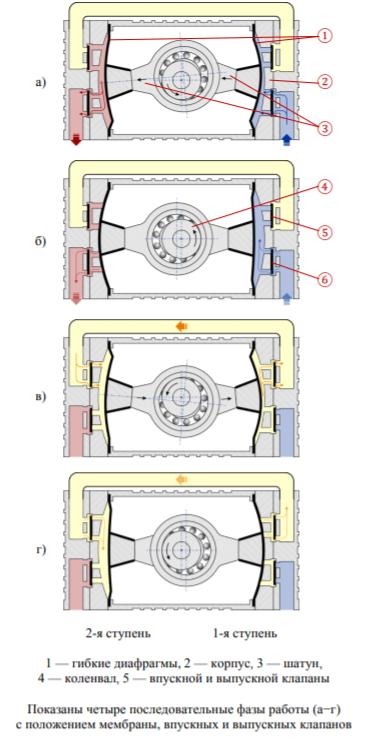
\includegraphics[width = 7.5 cm]{ДН}
    \caption{Работа диафрагменного насоса}
    \label{fig:vac}
\end{figure}

\textbf{Преимущества}: отсутствие материалов, загрязняющих рабочий
объем насоса и, как следствие, откачиваемый объем: масла, других смазочных веществ, трущихся механизмов; используется для предварительной (форвакуумной откачки) в системах безмасляной (т.н. «сухой») откачки с особым требованием чистоты откачиваемого объема; используется до 4-х последовательных ступеней; низкий уровень шума.

\textbf{Недостатки}: низкая скорость откачки за счет ограниченной эластичности диафрагмы; низкий предельный вакуум за счет обратного потока воздуха через выпускные клапаны; ограниченность срока службы
сроком функционирования диафрагмы.

\textbf{Тип вакуума}: средний.

\subsection{Турбомолекулярный насос}

\begin{figure}[h]
    \centering
    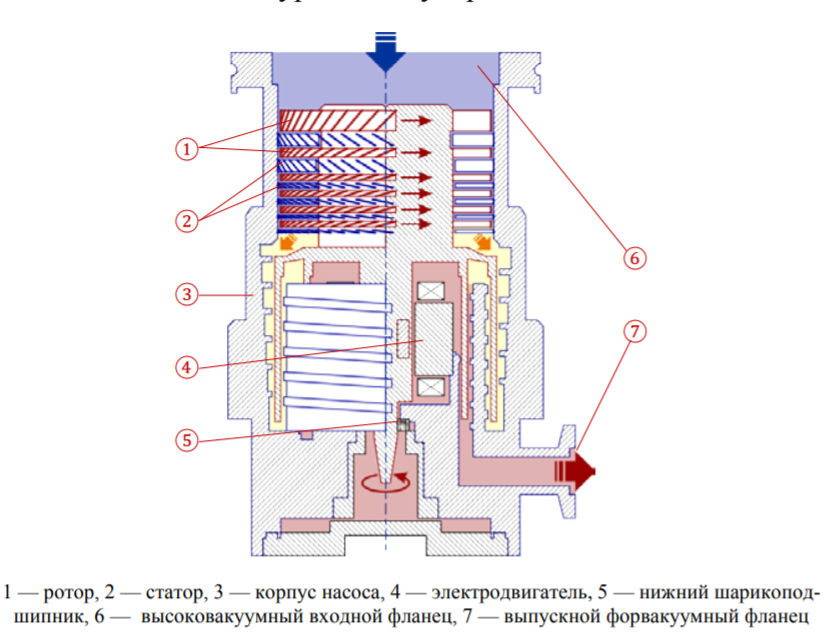
\includegraphics[width = 12 cm]{ТМН}
    \caption{Конструкция турбомолекулярного насоса}
    \label{fig:vac}
\end{figure}

Откачка в турбомолекулярном насосе осуществляется за
счет соударения частиц газа с быстродвижущимися турбинными лопатками дисков ротора (1) специальной геометрии, которые придают им дополнительный импульс в заданном направлении потока. Между дисками ротора находятся диски статора (2) с обратно обращенными лопатками, направляющие поток молекул на следующие диски турбины по оптимальной траектории, минимизируя обратный поток. Каждая пара пластин ротора-статора образует одну ступень. Насос состоит из нескольких ступеней расположенных последовательно, каждая последующая ступень имеет меньшие геометрические размеры, что при постоянном потоке
газа приводит к постепенному повышению давления до выпускного форвакуумного. Скорость вращения ротора современных турбомолекулярных
насосов достигает нескольких десятков тысяч оборотов в минуту.

\begin{figure}[h]
    \centering
    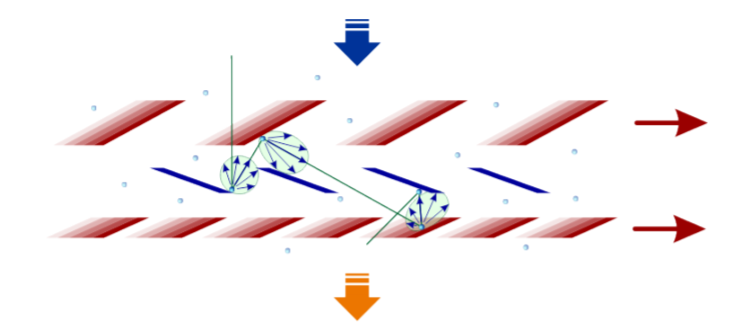
\includegraphics[width = 10.5 cm]{Принцип ТМН}
    \caption{Принцип работы турбомолекулярного насоса}
    \label{fig:vac}
\end{figure}

\textbf{Преимущества}: постоянная готовность к работе; быстрый запуск($\thicksim 10$ минут на раскручивание турбины); устойчивость к резкому повышению давления (вплоть до атмосферного); широкий диапазон рабочих давлений ($10^{-7}$ - $10^{-1}$ Па); примерно одинаковая быстрота действия для большинства газов; используется как в системах «сухой» безмасляной откачки с особым требованием чистоты откачиваемого объема, так и с масляными форвакуумными насосами за счёт минимального обратного потока.

\textbf{Недостатки}: требуется надежная защита вращающейся турбины от любых механических воздействий (пыли, абразивных частиц, вибраций, частых и резких перепадов давления и т. п.), приводящих к износу подвески ротора и разрушению лопаток турбины.

\textbf{Тип вакуума}: высокий.


\subsection{Терморезисторный вакуумметр (Пирани)}

Принцип действия тепловых манометров основан на зависимости
теплопроводности газа от давления. Чувствительным элементом терморезисторного датчика является тонкая металлическая нить накала (вольфрам, платина), помещенная в атмосферу откачиваемого газа. Сопротивление нити зависит от её температуры. Нить включена в одно из плеч мостовой схемы и разогрета до нескольких сотен градусов пропускаемым по ней током. Джоулево тепло, выделяемое нитью, отводится в основном через газовую среду со скоростью, зависящей от коэффициента теплопроводности. В зависимости от способа измерения вакуумметр работает в режиме (а) поддержания постоянного сопротивления моста (а значит и температуры нити), (б) постоянного напряжения на клеммах $А$, $С$ моста или (в) постоянного тока через мост. Мост изначально сбалансирован при давлении много ниже рабочего диапазона (сопротивление $R_{\text{Б}}$).

\begin{figure}[h]
    \centering
    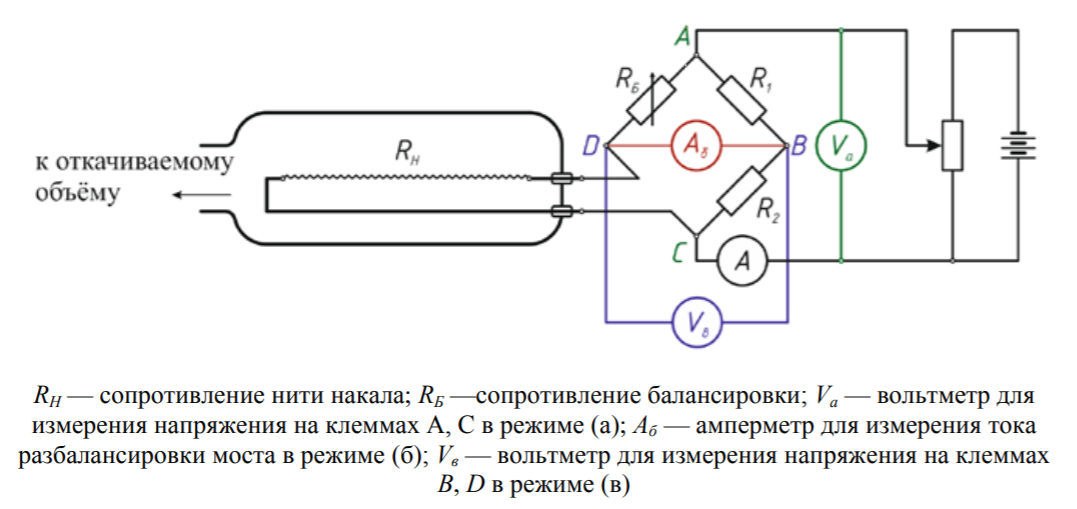
\includegraphics[width = 13 cm]{Пирани}
    \caption{Принципиальная схема терморезисторного вакуумметра (Пирани)}
    \label{fig:vac}
\end{figure}

В первом случае (а) напряжение на клеммах $А$, $С$ моста автоматически подбирается так, чтобы мост всё время оставался сбалансированным при изменении давления и, тем самым, является мерой давления в системе: 

\begin{equation}
	P \thicksim V^2 - V_{0}^2
\end{equation}
где $V_0$ -- — напряжение на клеммах при начальной балансировке.
Во втором случае (б) мерой давления служит ток разбалансировки моста, в третьем (в) — напряжение на клеммах $B$, $D$. 

В области низкого вакуума при $\lambda \gg d$ коэффициент теплопроводности перестаёт зависеть от давления, а при давлениях менее $10^{-3}$ Торр
основную роль в процессе теплоотвода начинает играть излучение. Оба эти фактора ограничивают применение данного типа датчиков областью среднего вакуума.

\textbf{Преимущества}: практически неограниченный срок службы
в неагрессивных средах за счёт низкой степени окисления нити
при низких температурах нагрева. Способность выдержать прорыв атмосферы.

\textbf{Недостатки}: при давлениях более $1$ мбар показания существенно
зависят от типа газа; тепловая инерция — запаздывание показаний при резком изменении давления; необходимость перекалибровки датчика в связи с изменением сопротивления после длительного времени эксплуатации.

\textbf{Тип вакуума}: средний.


\subsection{Магнетронный вакуумметр (с холодным катодом)}

Измерительный объём магнетронного датчика находится
между катодом и анодом, между которыми приложено напряжение
($\thicksim 2-6$ кВ), а также помещен в постоянное магнитное поле ($\thicksim 0,2-2$ кГс).
Случайным образом возникшие вблизи катода электроны (например,
вследствие автоэлектронной эмиссии) будут двигаться к аноду под действием скрещенных электромагнитных полей по удлиненной траектории. При этом повышается вероятность соударения электронов с молекулами откачиваемого газа и их ионизация. Образовавшиеся ионы ускоряются в электрическом поле анодно-катодного промежутка и выбивают из материала катода вторичные электроны (вторичная электронная эмиссия), которые также ионизируют газ, двигаясь к аноду по сложной циклической траектории.

В результате описанного процесса возникает электрический разряд, ток которого в достаточно широком диапазоне зависит от давления.
На диапазон измеряемых давлений существенно влияет конструкция магнетронного датчика. В инверсно-магнетроном датчике анодом служит центральный металлический стержень, а катодом — осесимметричная
обечайка, магнитное поле создается внешним постоянным кольцевым
магнитом.

\begin{figure}[h]
    \centering
    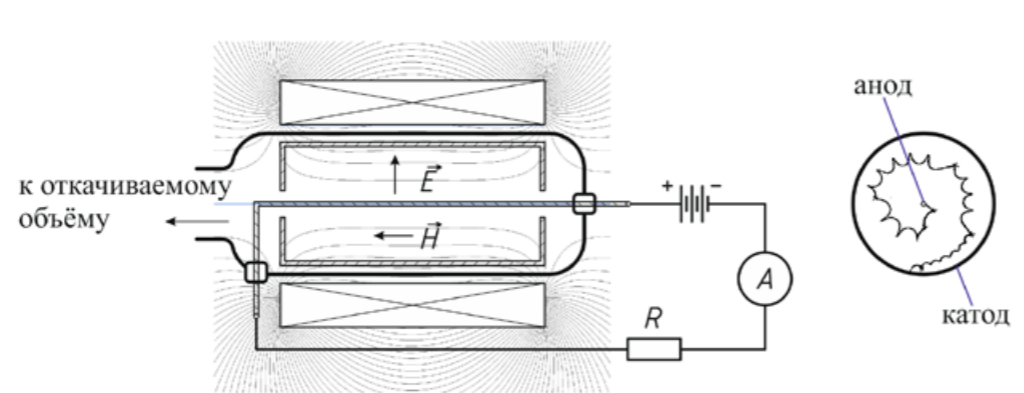
\includegraphics[width = 13 cm]{Магнетрон}
    \caption{Принципиальная схема инверсно-магнетронного вакуумметра и траектории электронов в них}
    \label{fig:vac}
\end{figure}

\textbf{Преимущества}: могут включаться в широком диапазоне давлений, т.к. не содержат накаленных деталей и не боятся окисления. Устойчивы к прорыву атмосферы. Применяются в автоматизированных технологических процессах вследствие простоты эксплуатации
и нечувствительности к внешним воздействиям.

\textbf{Недостатки}: Не желательно длительное использование в диапазоне среднего вакуума особенно в атмосфере аргона, т.к. это приводит к распылению материала катода потоком ионов, что, в свою очередь, может стать причиной короткого замыкания и сбоев датчика. Не желательно использование в системах с масляным типом откачки, т.к. углеводороды со временем образуют устойчивую пленку на поверхности катода, которая искажает показания датчика. Является источником магнитного поля, что может влиять на работу других приборов.

\textbf{Тип вакуума}: высокий, сверхвысокий.

\subsection{Рабочая установка}

\begin{figure}[h]
    \centering
    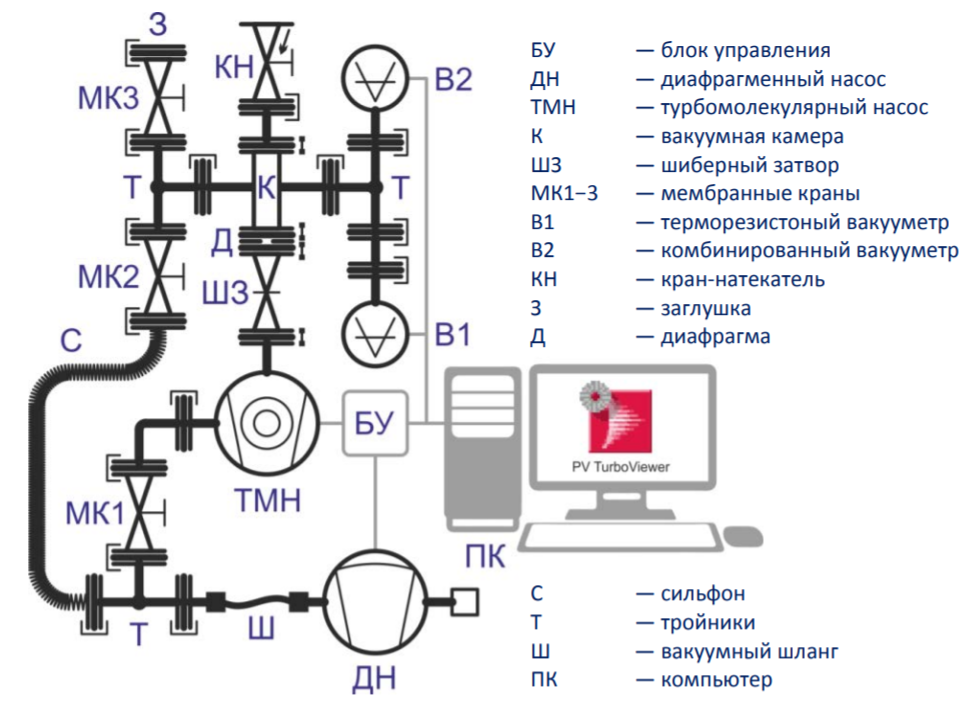
\includegraphics[width = 13 cm]{Схема}
    \caption{Схема экспериментального стенда}
    \label{fig:vac}
\end{figure}

Экспериментальный стенд выполнен на основе компактного безмасляного высоковакуумного откачного поста Pfeiffer Vacuum серии HiCube 80 Eco с диафрагменным и турбомолекулярным насосами, вакуумметров Pfeiffer Vacuum серии DigiLine, и вакуумных быстроразъёмных компонентов. Управление основными функциями откачного
поста, контроль и запись параметров установки осуществляется блоком управления (БУ) через цифровой интерфейс RS-485 с помощью специального программного обеспечения PV TurboViewer.

\begin{figure}[h]
    \centering
    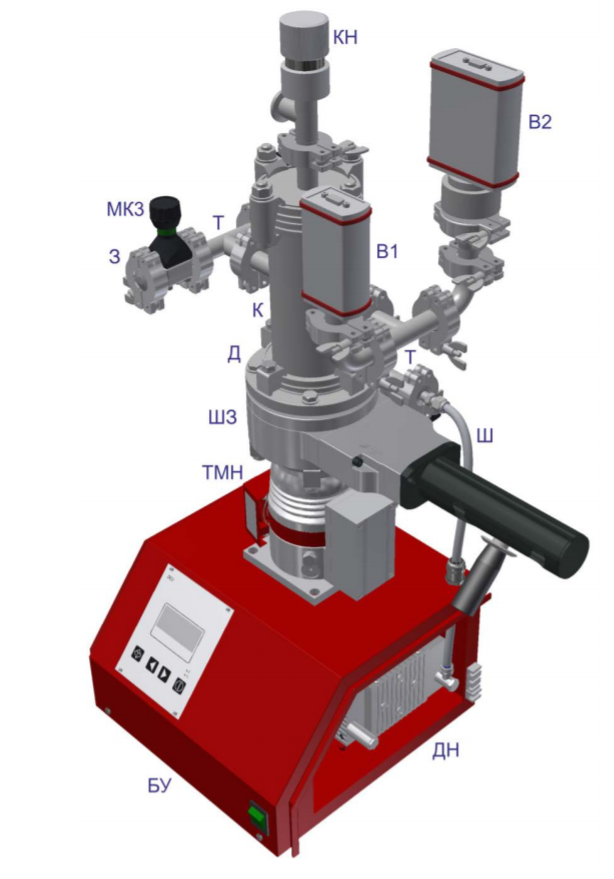
\includegraphics[width = 10.5 cm]{Внешний вид}
    \caption{Внешний вид экспериментального стенда}
    \label{fig:vac}
\end{figure}


\section{Измерения и обработка данных}
\subsection{Подготовка к работе и подключение системы управления}

Для начала работы с экспериментальной установкой подготовим всё для снятия измерений. Для этого подготовим все краны, предврательно открыв их, далее включим программу на компьютере, управляющую насосами и вакууметрами. 

\subsection{Определение откачиваемого объёма и измерение скорости откачки форвакуумным насосом}

Для обработки данных необходимо знать объёмы кранов установки. 
Для определения объемов частей установки (объем вакуумной камеры -- $V_{K},$  объем форвакуумной магистрали + объем ТМН -- $V_{\text{ф.м. + тмн}}$ воспользуемся законом Бойля-Мариотта. Для этого необходимо определить давления в различных состояниях установки (исследовать различные части установки).

Присоединяя часть известного объёма к установке, можно измерить давление до и после, из закона Бойля-Мариотта получить сам объём кранов установки.

Для этого проделаем следующее:
\begin{enumerate}
	\item Откачаем установку форвакуумным насосом ДН.
	\item Присоединим к установке сильфон с воздухом при атмосферном давлении.
	\item Выравним давления в сильфоне С и вакуумной камере К экспериментального стенда.
	\item Выравним давление вакуумной камеры К и форвакуумной магистрали установки.
	\item Выравним давление во всей установке, включая объем турбомолекулярного насоса ТМН.
	\item Зафиксируем установившиеся показания вакуумметров.
	
\end{enumerate}
	
На каждом этапе выравнивания давления фиксируем его. Для лучшей точности было проведено 3 измерения, результаты которых занесены в таблицу. Значения погрешностей определяются с формул погрешностей прямых измерений.

\begin{table}[h]
	\begin{center}
		\begin{tabular}{|c|c|c|c|c|c|}
		\hline
		\multicolumn{2}{|c|}{1} & \multicolumn{2}{c|}{2} & \multicolumn{2}{c|}{3} \\ \hline
		$p$, мбар  & $\sigma_{p}$, мбар & $p$, мбар & $\sigma_{p}$, мбар & $p$, мбар & $\sigma_{p}$, мбар \\ \hline
		3,2     & 0,08         & 3,5    & 0,06         & 3,2 & 0,03         \\ \hline
		190      & 3            & 196     & 5            & 194     & 6            \\ \hline
		140      & 3            & 144     & 5            & 145     & 6            \\ \hline
		\end{tabular}
		\caption{Результаты измерения давления при различных конфигурациях системы.}
	\end{center}
\end{table}

Используя закон Бойля-Мариотта, получаем соотношения:

\begin{equation}
		V_{K} = \frac{p_{\text{атм}} - p_{2}}{p_{2} - p_{1}} V_{\text{сильф}};
		\label{eq:value_of_vacuum_cam}
\end{equation}
	
\begin{equation}
		V_{\text{ф.м. + тмн}} = \frac{ \left( p_{3} - p_{2}\right) \left( V_{K} + V_{\text{сильф}}\right) }{p_{1} - p_{3}};
		\label{eq:value_of_forvacuum_tube}
\end{equation}

Используя соотношения (\ref{eq:value_of_vacuum_cam}, \ref{eq:value_of_forvacuum_tube}) определим объемы составных частей установки, а также погрешности косвенных измерений данных величин. Значения занесем в таблицу (\ref{tab:resultsof_measuring_for_diffrent_part_value}). В проделанном эксперименте значение объёма сильфона $V_{\text{сильф}}$ = 265 мл.

\begin{table}[h]
	\begin{center}
		\begin{tabular}{|c|c|c|c|c|}
		\hline
		Измерение & $V_{K}, cm^{3}$ & $\sigma_{V_{K}}, cm^{3}$ & $V_{\text{ф.м. + тмн}}, cm^{3}$ & $\sigma_{V_{\text{ф.м. + тмн}}}, cm^{3}$ \\ \hline
		1 & 1149 & 40 & 517 & 17 \\ \hline
		2 & 1107 & 55 & 508 & 26 \\ \hline
		3 & 1120 & 60 & 479 & 39 \\ \hline
		\end{tabular}
	\end{center}
	\caption{Результаты измерения объемов составных частей установки с погрешностью косвенного измерения}
						\label{tab:resultsof_measuring_for_diffrent_part_value}
\end{table}

Для объёмов имеем:

\begin{equation}
	V_{K} = 1125 \; \text{мл, }	\Delta V_{K} = 49 \; \text{мл}
\end{equation}

\begin{equation}
	V_{\text{ф.м. + тмн}} = 501 \; \text{мл, }	\Delta V_{\text{ф.м. + тмн}} = 27 \; \text{мл}
\end{equation}

\subsection{Измерение скорости откачки турбомолекулярным насосом}

Теперь проделаем следующее:

\begin{enumerate}
	\item Отсоединим сильфон от установки.
	\item Откачаем установку форвакуумным насосом ДН.
	\item Откачаем объём турбомолекулярным насосом ТМН.
	\item Видно, что терморезисторный вакуумметр $В1$ достиг своего предела измерений, в то время как комбинированный вакуумметр $В2$ (точнее его магнетронная часть) продолжает отображать корректное давление в системе. Зафиксируйте предельное давление в высоковакуумной части установки и время откачки установки насосом ТМН.
	\item Определим уровень течей и скорость откачки системы. Для этого закроем шибер ШЗ, при этом давление в системе начнёт повышаться за счёт наличия течей. Получим таким образом зависимость показаний вакууметра $В2$ от времени. Когда давление превысит $3 \cdot 10^{-3}$ мбар,
снова откроем шибер. Получим зависимость показаний вакуумметра $В2$ от времени после открытия шибера. Снова зафиксируем предельное давление.
\end{enumerate}

Мы получили зависимость $P(t)$, отсюда строим график $ln(P)(t)$ и находим параметры полученной кривой методом МНК:

\begin{figure}[h]
    \centering
    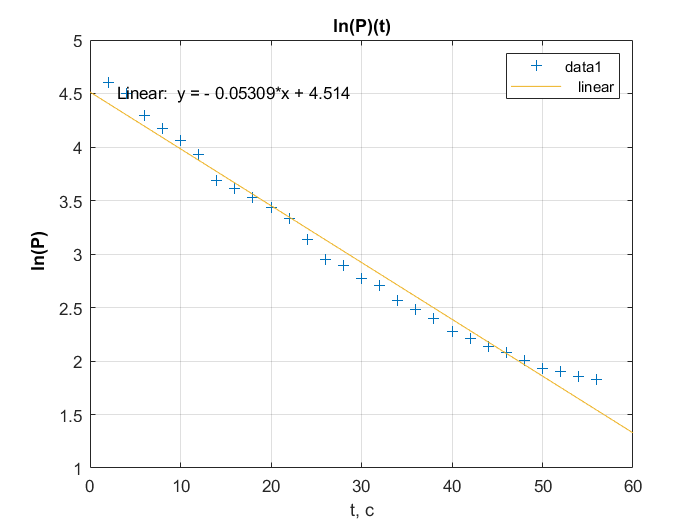
\includegraphics[width = 11 cm]{fig1}
    \caption{График зависимости $ln(P)(t)$ для ДН}
    \label{fig:vac}
\end{figure}

\begin{equation}
	\tau = 18,83 \; \text{с, } \Delta \tau = 0,42 \; \text{с}
\end{equation}

Отсюда легко находим следующее ($S_{\text{н}} = 138,9 \; \text{мл/с}$)

\begin{equation}
	S_{\text{o}} = \frac{V_{\text{o}}}{\tau} = \frac{V_{\text{К}}}{\tau} = 59,75 \; \text{мл/с}
\end{equation}

\begin{equation}
	\Delta S_{\text{o}} = \frac{\Delta V_{\text{К}}}{\tau} + \frac{\Delta \tau V_{\text{К}}}{\tau^2} = 3,93 \; \text{мл/с}
\end{equation}

\begin{equation}
	U = \frac{S_{\text{н}} S_{\text{o}}}{S_{\text{н}} - S_{\text{o}}} = 104,86 \; \text{мл/с}
\end{equation}

\begin{equation}
	\Delta U = 6,89\; \text{мл/с}
\end{equation}


\subsection{Измерение влияния течи на вакуум}

Проделывая аналогичные действия откачки с помощью ТМН, получим следующий график зависимости (для того, чтобы убедиться в повторяемости результатов, на самом деле было проделано 3 эксперимента, которые имеют одинаковый результат):

\begin{figure}[h]
    \centering
    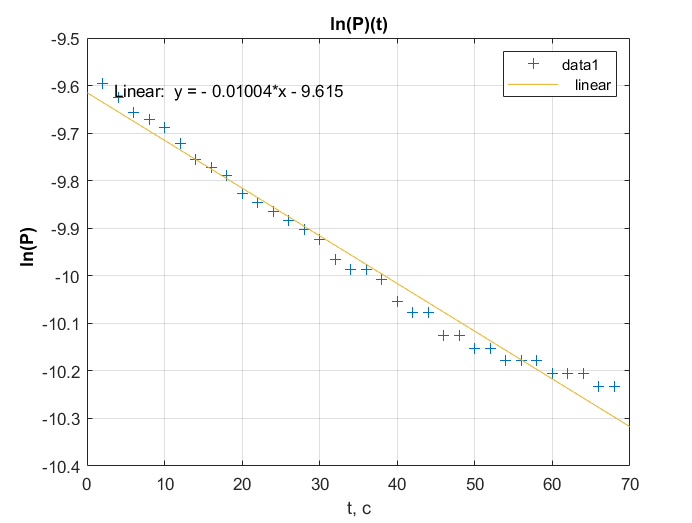
\includegraphics[width = 11 cm]{fig2}
    \caption{График зависимости $ln(P)(t)$ для ТМН}
    \label{fig:vac}
\end{figure}

\begin{equation}
	\tau = 103,24 \; \text{с, } \Delta \tau = 8,93 \; \text{с}
\end{equation}

Отсюда легко находим следующее ($S_{\text{н}} = 138,9 \; \text{мл/с}$)

\begin{equation}
	S_{\text{o}} = \frac{V_{\text{o}}}{\tau} = \frac{V_{\text{К}}}{\tau} = 10,30 \; \text{мл/с}
\end{equation}

\begin{equation}
	\Delta S_{\text{o}} = \frac{\Delta V_{\text{К}}}{\tau} + \frac{\Delta \tau V_{\text{К}}}{\tau^2} = 1,11 \; \text{мл/с}
\end{equation}

\begin{equation}
	U = \frac{S_{\text{н}} S_{\text{o}}}{S_{\text{н}} - S_{\text{o}}} = 10,31 \; \text{мл/с}
\end{equation}

\begin{equation}
	\Delta U = 1,28 \; \text{мл/с}
\end{equation}

В данном случае $S_{\text{н}} \gg S_{\text{о}}$.

Сравним полученное значение с оценкой, выведенной для проводимости отверстия:

\begin{equation}
	U_{\text{{отв}}} = \frac{Av}{4} = \frac{\pi R^2}{4} \sqrt{\frac{8kT}{\pi m}} \thicksim 30 \; \text{мл/с}
\end{equation}

Порядок величин совпадает, значит полученное значение имеет смысл. В оценке были использованы радиус $R = 1$ см и температура $T = 300$ К.

Определим уровень течей по ухудшению вакуума после перекрытия откачки насосом ТМН. Для этого удобно взять часть графика, где соблюдается линейная зависимость.  

\begin{figure}[h]
    \centering
    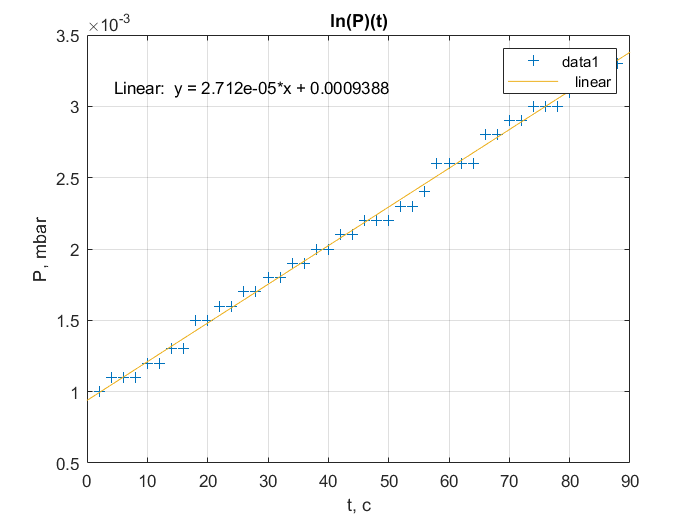
\includegraphics[width = 11 cm]{fig3}
    \caption{График зависимости $ln(P)(t)$ для ТМН}
    \label{fig:vac}
\end{figure}

\begin{equation}
	Q_{\text{н}} = V \frac{dP}{dt} = 0,030 \; \text{мл} \cdot \text{мбар/c} \ll P S_{\text{о}}
\end{equation}

Проверка показывает, что в данном случае $Q_{\text{н}} \ll Q$, что является допустимым значением уровня течей по ухудшению вакуума. (Давление берём среднее из графика в качестве оценки).

Заметим, что результаты получились довольно близки к теоретическим значениям.

\subsection{Проверка используемой модели течения}

Оценим число Кнудсена для предельных давлений после использования ДН и ТМН для создания вакуума, зная, что диаметр молекул воздуха равен $0,365$ нм.

\begin{equation}
	Kn = \frac{\lambda}{d} \thicksim \frac{1}{\sqrt{2} \sigma n \sqrt[3]{V}} = \frac{kT}{\sqrt{2} \sigma p \sqrt[3]{V}}
\end{equation}

\begin{equation}
	Kn_{\text{ДН}} = 8 \cdot 10^{-4}
\end{equation}

\begin{equation}
	Kn_{\text{ТМН}} = 300
\end{equation}

Видно, что при первом значении давления реализуется гидродинамический режим течения, а уже при втором значении молекулярный режим течения.

\section{Заключение}

В результате проделанного эксперимента были изучены основные современные способы получения вакуума, изучены численные характеристики используемых насосов, а также определены скорости откачки системы в стационарном режиме и по ухудшению и улучшению вакуума.


\section{Список используемой литературы}

$\bullet$ \href{https://mipt.ru/education/chair/physics/S_II/lab/}{Описание лабораторных работ на кафедре общей физики МФТИ}






 
\end{document}